\begin{figure}[t!]
    \centering
    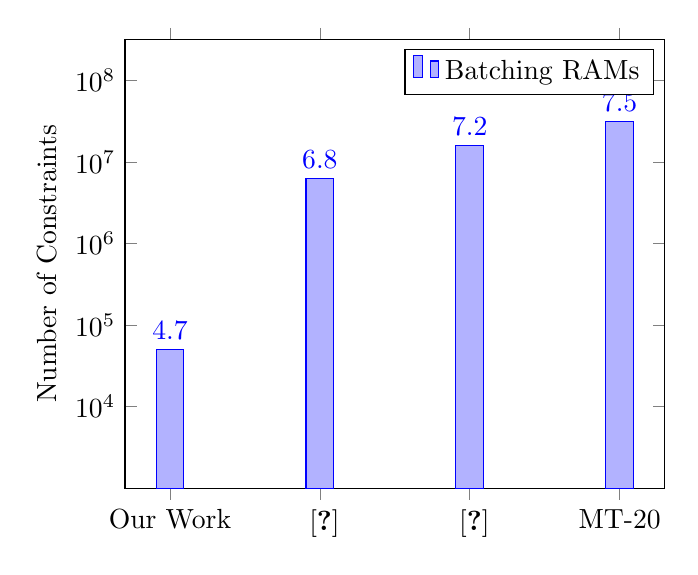
\begin{tikzpicture}
        \begin{axis}[
        ybar,
        ylabel={Number of Constraints},
        ymin = 3,
        ymax = 8.5,
        ytick = {4, 5, 6, 7, 8},
        xlabel={},
        xtick=data,
        symbolic x coords= {A, B, C, D},
        xticklabels = {{Our Work}, ~\cite{CCS:CFHKKO22}, ~\cite{USENIX:OWWB20}, MT-20},
        yticklabels = {$10^4$, $10^5$, $10^6$, $10^7$, $10^8$},
        xlabel near ticks,
        ylabel near ticks,
        nodes near coords,
        nodes near coords align={vertical},
        ]
        \addplot coordinates {(A,4.7) (B,6.8) (C,7.2) (D,7.5)};
        \legend{Batching RAMs}
        \end{axis}

    \end{tikzpicture}
    \caption{Comparison of Constraints incurred by different approaches for batching RAMs. MT-20
    refers to Merkle-tree with depth 20.}
    \label{fig:batch-ram-constraints}
\end{figure}

\begin{figure}[t!]
    \centering
    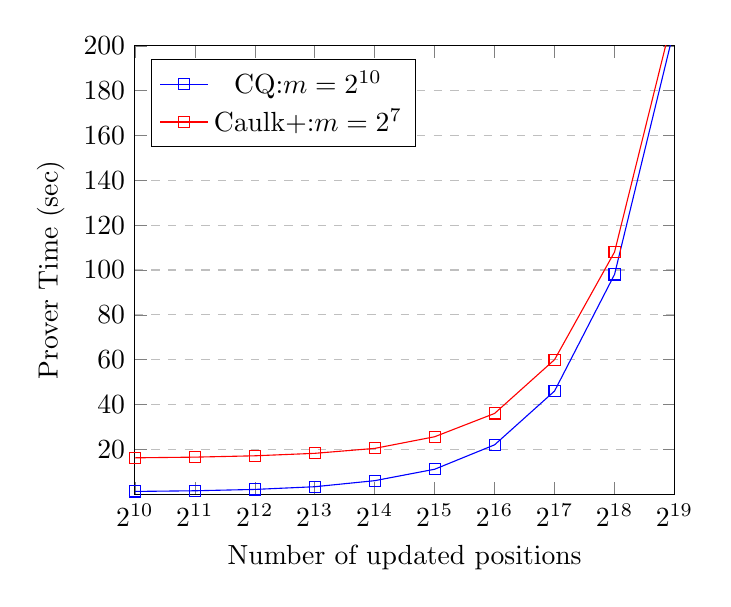
\begin{tikzpicture}
        \begin{axis}[
        xmin=0,
        xmax=9,
        ymin=0,
        ymax=200,
        xlabel={Number of updated positions},
        ylabel={Prover Time (sec)},
        xtick={0, 1, 2, 3, 4, 5, 6, 7, 8, 9},
        ytick={20, 40, 60, 80, 100, 120, 140, 160, 180, 200},
        xticklabels={$2^{10}$, $2^{11}$, $2^{12}$, $2^{13}$, $2^{14}$, $2^{15}$, $2^{16}$, $2^{17}$, $2^{18}$, $2^{19}$},
        yticklabels={20, 40, 60, 80, 100, 120, 140, 160, 180, 200},
        legend pos=north west,
        ymajorgrids=true,
        grid style=dashed,
        xlabel near ticks,
        ylabel near ticks
        ]
        \addlegendimage{color=blue, mark=square}
        \addlegendentry{CQ:$m=2^{10}$}
        \addlegendimage{color=red, mark=square}
        \addlegendentry{Caulk+:$m=2^{7}$}
        \addplot[
            color=blue,
            mark=square,
        ]
        coordinates {
            (0,1.2)(1,1.5)(2,2.1)(3,3.3)(4,6.0)(5,11.1)(6,22.0)(7,46)(8,98)(9,208)
        };

        \addplot[
            color=red,
            mark=square,
        ]
        coordinates {
            (0,16.2)(1,16.5)(2,17.1)(3,18.2)(4,20.4)(5,25.6)(6,36)(7,60)(8,108)(9,216)
        };
        \end{axis}
    \end{tikzpicture}
    \caption{Online Prover Performance of our Batching-Efficient RAM with updates}
    \label{fig:batch-ram-proving-time}
\end{figure}

In this section we report on the experimental evaluation of our batching-efficient RAM.
In addition, we also report on the overhead (as a function of changes since last parameter computation)
incurred by our updatable lookup arguments over the vanilla lookup arguments with read-only table. We
benchmark this overhead over vanilla implementations of Caulk+ ~\cite{EPRINT:PosKat22} and
CQ ~\cite{EPRINT:EagFioGab22}, both of which we also implement (as their non zero-knowledge variants)
for our evaluation. Our implementation is built on top of existing implementation ~\cite{caulk-implementation}
of lookup argument Caulk ~\cite{CCS:ZBKMNS22}. We make our implementation available at
\url{https://anonymous.4open.science/r/updatableRAM/} for anonymous submission. We later plan to
make the implementation available as open-source project.
All the benchmarks were run single-threaded on a commodity configuration featuring a $2.1GHz$ Intel-I5 processor,
$16$ GB memory running Ubuntu Linux 22.04. The implementation was compiled using {\tt --release}
flag in Rust. Generating table specific parameters for table of size $1$ million takes around $12,000$
seconds for CQ based instantiation.

We first provide overall running time of batching-efficient RAM primitive instantiated with Caulk+
and CQ lookup arguments. The degradation in running time is plotted as function of accumulated updates
since the last computation of full table-specific parameters in Figure ~\ref{fig:batch-ram-proving-time}.
We choose batch size of $m=128$ for Caulk+ based instantiation (to avoid prohibitive performance),
while we consider $m=1024$ for CQ based instantiation. Our overhead remains barely noticable against
the quadratic costs incurred by Caulk+ base protocol till about $2^{15}$ accumulated changes, equivalent of
$128$ lookups of size $512$. While the performance overhead compared to base CQ protocol is much more apparent,
overall we continue to achieve online proof generation time of under a minute all the way upto
$\approx 2\times 10^5$ accumulated changes, equivalent of roughly $200$ batch updates (assuming the worst-case
scenario). In real application scenarios, we can expect better degradation curve, as its unlikely that updates
to the table occur uniformly across all positions.

In Figure ~\ref{fig:batch-ram-constraints}, we compare the
R1CS constraints incurred by existing approaches to batching friendly RAMs/accumulators. For our work, we assume
that the memory checking on the RAM instance of size $m$ is implemented as an arithmetic circuit using a Bene's
routing network ~\cite{benes}, though we also provide a purely polynomial protocol for the same in Section ~\ref{sec:poly-proto-ram-app}.
Our construction is relatively ``circuit-free'' and relies on the efficiency of lookup arguments coupled with
our novel modifications to make them update resilient.

Finally, we also compare the efficacy of our quasi-linear algorithm to compute scalar coefficients in
Lemma ~\ref{lem:sum-computation}, required to assemble the encoded quotients from pre-computed quotients.
This algorithm is implemented and tested in the {\tt fastupdate} module of the referenced repository.
In Table ~\ref{tbl:sum-computation-compare}, we compare it against the naive computation of the quotients.
In the table, we vary the sizes of set $I$ in Lemma ~\ref{lem:sum-computation} in the set $\{2^i:7\leq i\leq 10\}$
and set $K=2^7|I|$, i.e, we compare the two methods to sustain $\approx 100$ online proofs. We clearly see
$5\times-20\times$ advantage over the naive computation.

\begin{table}[htbp]
    \centering
    \begin{tabularx}{0.45\textwidth}{@{}XXXX@{}}
        \toprule
         $|I|$ & $|K|$ & Lemma ~\ref{lem:sum-computation} & Naive \\ \midrule
        $2^7$ & $2^{14}$ & 3.3s  & 12s \\
        $2^8$ & $2^{15}$ & 7.7s  & 48s \\
        $2^9$ & $2^{16}$ & 16.8s & 198s \\
        $2^{10}$ & $2^{17}$ & 39.2s & 839s \\
        \bottomrule
    \end{tabularx}
    \caption{Comparison of Lemma ~\ref{lem:sum-computation} and naive computation for calculating
    scalar coefficients for encoded quotients.}
    \label{tbl:sum-computation-compare}
\end{table}

\smallskip

\noindent{\bf Continuity.} To maintain {\em continuity} of the system~(this is particularly important for applications such as rollups), we must carefully
align the online prover performance curve with the cost of offline computation.  As an example, suppose $\vec{T}_0$
is the initial pre-processed table at time $t=0$. We generate proofs using pre-computed parameters for $\vec{T}_0$
till the time $t=t_1$, when the table state $\vec{T}_1$ is at hamming distance $2^{17}$ from $\vec{T}_0$. At this point,
from Figure ~\ref{fig:batch-ram-proving-time}, online proof generation takes around $40s$ for batch of $1000$ updates.
At $t=t_1$, we also start an offline parameter computation for the table $\vec{T}_1$, while continuing to generate
online proofs using parameters for $\vec{T}_0$. We can generate the next $2^7$ batches of updates at an average of
approximately $12000/128\approx 94s$ each, thus finishing with a table state $\vec{T}_2$ at hamming distance at most
$2^{18}$ from $\vec{T}_0$ at $t_2=t_1+12000$. At this point, we should have the pre-computed parameters for $\vec{T}_1$,
which is at update distance of $2^{17}$ from $\vec{T}_2$, and thus online proof generation can switch to parameters
for the table $\vec{T}_1$. This alignment gives us a proving time of $94s$ per batch of $1000$, while ensuring system
is live at all times. Clearly, a faster offline pre-computation using parallel implementation would allow us to stay
at the cheaper end of online proving performance.



